\documentclass[11pt]{article}
%\usepackage[firstpage]{draftwatermark}
\usepackage{times}
\usepackage{pdfpages}
\usepackage{fullpage}
\usepackage{url}
\usepackage{hyperref}
\usepackage{fancyhdr}
\usepackage{graphicx}
\usepackage{tabularx}
\usepackage{enumitem}
\usepackage{indentfirst}
\usepackage{subcaption}
\usepackage{amsmath, amsfonts, amsthm, fouriernc}

% Added by bsb
\usepackage{color,soul}
\DeclareRobustCommand{\hlr}[1]{{\sethlcolor{red}\hl{#1}}}
\DeclareRobustCommand{\hlg}[1]{{\sethlcolor{green}\hl{#1}}}
\DeclareRobustCommand{\hlb}[1]{{\sethlcolor{blue}\hl{#1}}}
\DeclareRobustCommand{\hly}[1]{{\sethlcolor{yellow}\hl{#1}}}


\setcounter{secnumdepth}{4}
\graphicspath{{images/}}
\pagestyle{fancy}

\newenvironment{xitemize}{\begin{itemize}\addtolength{\itemsep}{-0.75em}}{\end{itemize}}
\newenvironment{tasklist}{\begin{enumerate}[label=\textbf{\thesubsubsection-\arabic*},ref=\thesubsubsection-\arabic*,leftmargin=*]}{\end{enumerate}}
\newcommand\todo[1]{{\bf TODO: #1}}
\setcounter{tocdepth}{2}
\setcounter{secnumdepth}{4}

\addtolength{\headheight}{2em}
\addtolength{\headsep}{1.5em}
\rhead{ME 2801}


\begin{document}

\begin{center}
  \Huge{Gain}
\end{center}

In ME2801 we cover a number of topics in linear systems and feedback control.  In that context we use the term \emph{gain} in a generic way and the term \emph{DC gain} is used to refer to a specific property of linear systems.
%and \emph{frequency response gain} to refer to a specific properties of a linear system.

\section{Gain}

The term \emph{gain} is used generically to refer to a linear system with a constant transfer function.  A common example is the transfer function for a PID controller which we can write as
\[
\frac{U(s)}{E(s)} = K_p + \frac{K_i}{s} + K_d (s)
  \]
  where $K_p$, $K_i$ and $K_d$ are referred to as the proportional, integral and derivative gain values.  Another example is the simple block diagram shown in Figure~\ref{f:gainblock} where the output is the product of the input and the gain value $K$.

\begin{figure}[htb!]
\centering  
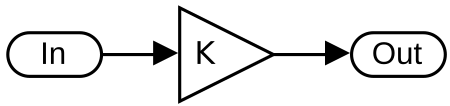
\includegraphics [width=0.25\textwidth]{gain_block.png}
\caption{Block diagram of gain.}
\label{f:gainblock}
\end{figure}

  
\section{DC Gain}

The \emph{DC gain}, $K_{dc}$, is a property of a system.  Considering a linear system described as a transfer function, the DC gain can be defined in either the time-domain or the frequency-domain.

\subsection{Time-Domain}
In the time-domain, the DC gain is the ratio of the magnitude of the steady-state step response to the magnitude of the step input.  Furthermore, if we consider a unit step response (where the input has a magnitude of one), then the DC gain is the steady-state magnitude of the output.  This property is illustrated in the second-order unity step response graphs of Figure~\ref{f:step}.  In the graph on the left, the input is amplified by a factor of 10 ($K_{dc}=10$).  In the graph on the right, the input is attenuated by a factor of 2 ($K_{dc}=0.5$).

\begin{figure}[hb!]
\centering  
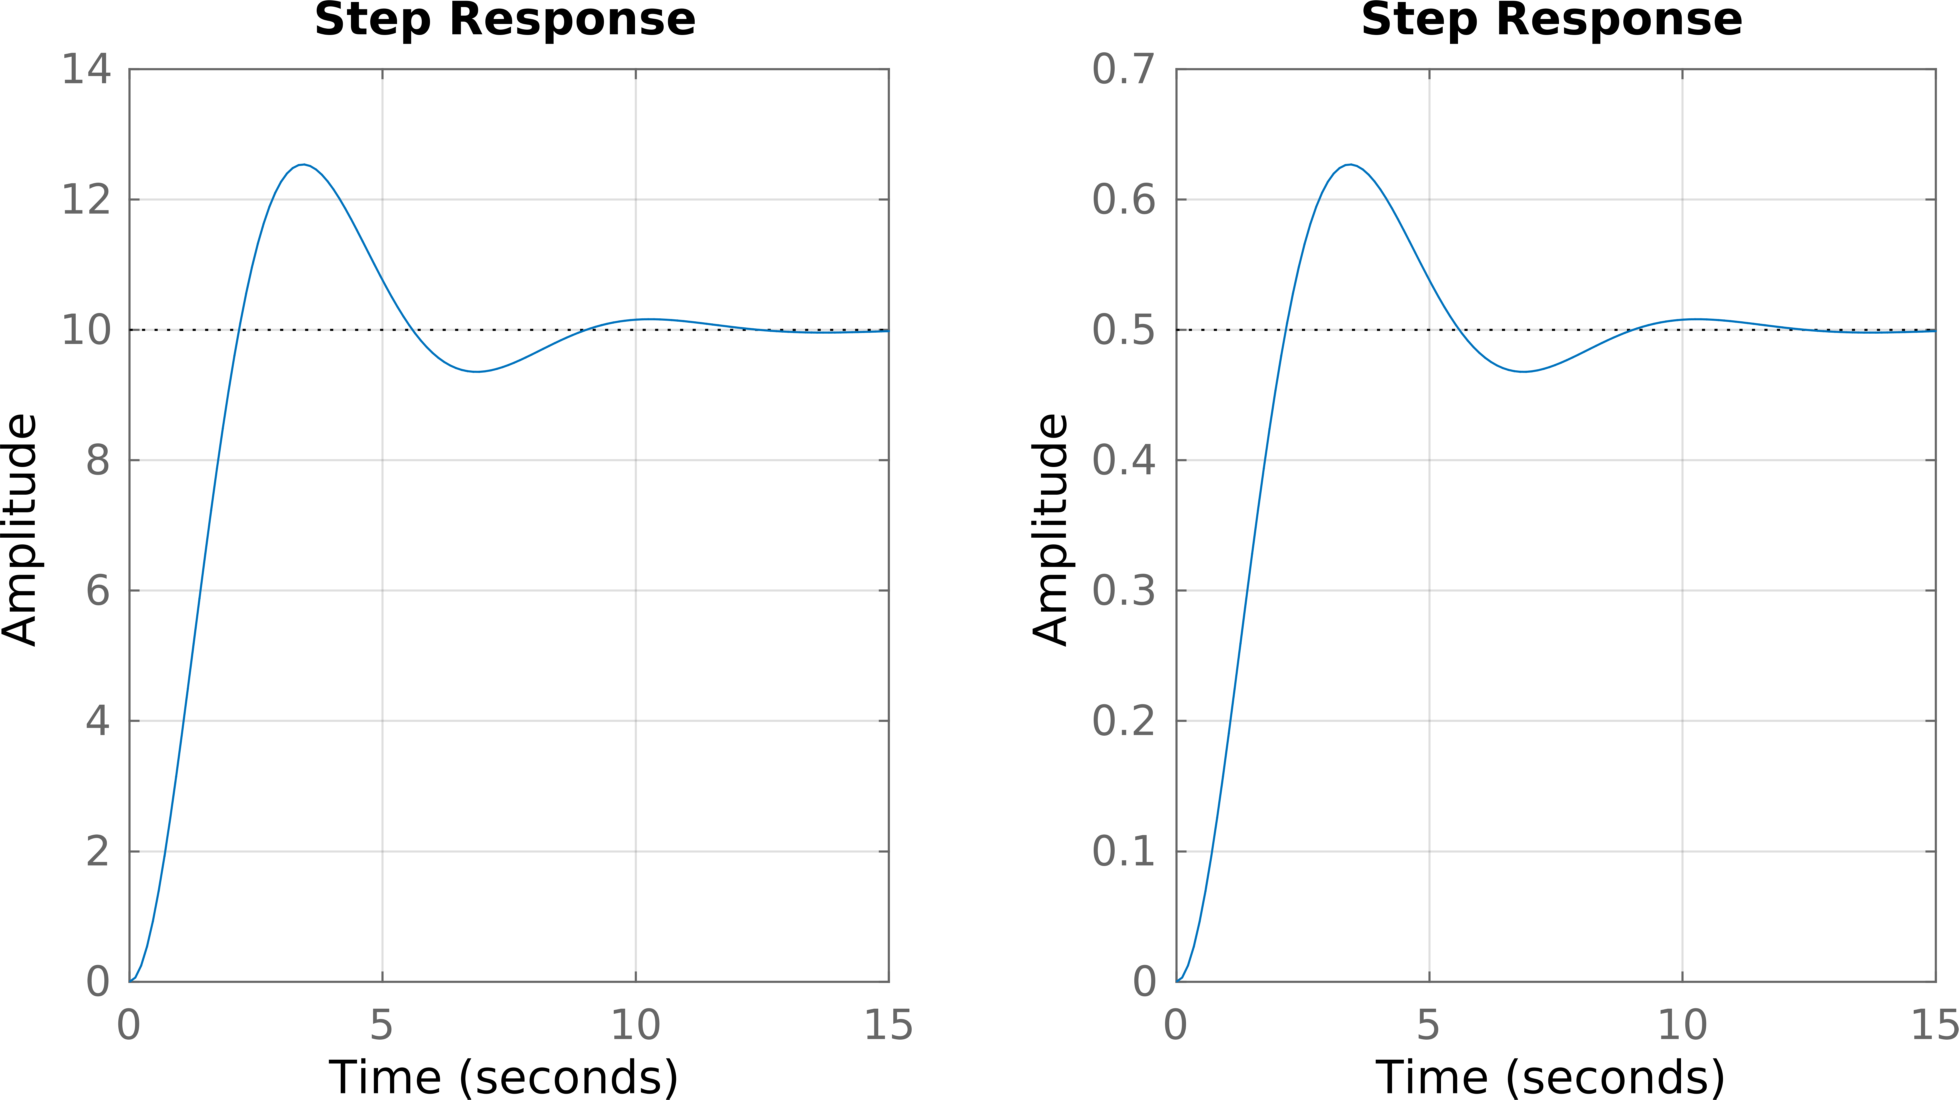
\includegraphics [width=0.6\textwidth]{step_gain.png}
\caption{Illustration of DC gain visible in the unity step response.  The system represented on the left has a DC gain of 10.  The system on the right has a DC gain of 0.5.}
\label{f:step}
\end{figure}

\subsubsection{DC Gain from Transfer Function}

Based on this time-domain definition of the DC gain, we can find the value directly from the transfer function
\[
\frac{Y(s)}{X(s)} = G(s).
\]
We consider the input to be a step input with a magnitude $X_0$, so $X(s) = \frac{X_0}{s}$.  Assuming a stable response, we can solve for the steady-state magnitude of the output $Y_0$ using the final value theorem which yields
\[
Y_0 = y(t \to \infty) = \lim_{s \to 0} \left[ s \, Y(s) \right]=  \lim_{s \to 0}  \left[ s \, G(s) \frac{X_0}{s} \right] =  \lim_{s \to 0} \left[ G(s) \right] X_0 = G(s=0) X_0.
\]
Since the DC gain is the ratio of output to input
\begin{equation}
  K_{dc} = \frac{Y_0}{X_0}  = \lim_{s \to 0} \left[ G(s) \right] = G(s=0).
  \label{e:dc_time}
\end{equation}

\subsection{Frequency-Domain}
In the frequency-domain, the DC gain is the magnitude of the ratio of output to input at zero frequency.  The magnitude of the transfer function is expressed as $|G(s=j\omega)|$, so the DC gain is
\begin{equation}
K_{dc}= \lim_{\omega \to 0} \left[ | G(j \omega) | \right] = G(s=0)
\end{equation}
which is equivalent to (\ref{e:dc_time}).

Using the Bode plot of a system, the DC gain is the value of the magnitude portion of the plot as the frequency approaches zero as illustrated in Figure~\ref{f:bode}.

\begin{figure}
\centering
\begin{subfigure}{.5\textwidth}
  \centering
  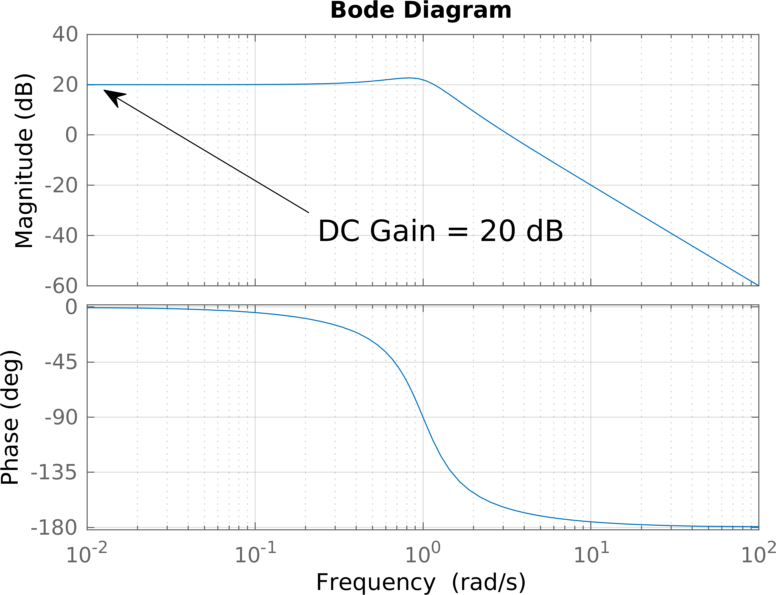
\includegraphics[width=\linewidth]{fig2.png}
  \caption{DC gain of 20 dB.}
  \label{fig:sub1}
\end{subfigure}%
\begin{subfigure}{.5\textwidth}
  \centering
  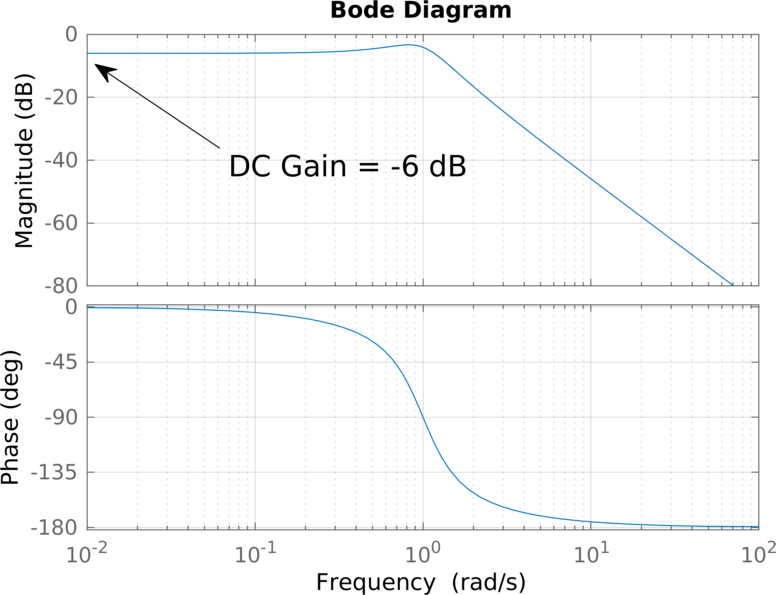
\includegraphics[width=\linewidth]{fig3.png}
  \caption{DC gain of -6 dB.}
  \label{fig:sub2}
\end{subfigure}
\caption{Illustration of DC gain visible in the frequency response (Bode plot) for the same two systems illustrated in Figure~\ref{f:step}.}
\label{f:bode}
\end{figure}

\subsection{Canonical Form of First and Second Order Transfer Functions}

In ME2801 we use standardized forms of the first and second order (underdamped) transfer functions:
\[
G_1(s) = K_{dc} \frac{a}{s+a} = K_{dc} \frac{1}{\tau \, s + 1}
\]
and
\[G_2(s) = K_{dc} \frac{\omega_n^2}{s^2 + 2 \zeta \omega_n s + \omega_n^2} = K_{dc} \frac{\omega_n^2}{(s+\zeta \omega_n)^2 + \omega_d^2}
\]
where $\omega_d = \omega_n \sqrt{1-\zeta^2}$. The reason for the particular forms of the expressions is that the gain term in each of the transfer functions above is equivalent to the DC gain ($K_{dc}$) as defined in (\ref{e:dc_time}).

\subsection{Exercises}

\begin{enumerate}
\item Find $K_{dc}$ for the the following transfer functions:
  \begin{enumerate}
  \item $\displaystyle G(s) = \frac{K}{s+a}$
  \item $\displaystyle G(s) = \frac{K}{s^2+2 \zeta \omega_n s + \omega_n^2}$
  \item $\displaystyle G(s) = \frac{K}{(s+\zeta \omega_n)^2+\omega_d^2}$
  \end{enumerate}
\item Given the second-order unit-step response in Figure~\ref{f:step2}, find $K_{dc}$, sketch the Bode plot and approximate the system transfer function.
  \item Given the Bode plot in Figure~\ref{f:bode2}, find $K_{dc}$, sketch the unit step response and approximate the system transfer function.
\end{enumerate}



\begin{figure}
\centering
\begin{subfigure}{.5\textwidth}
  \centering
  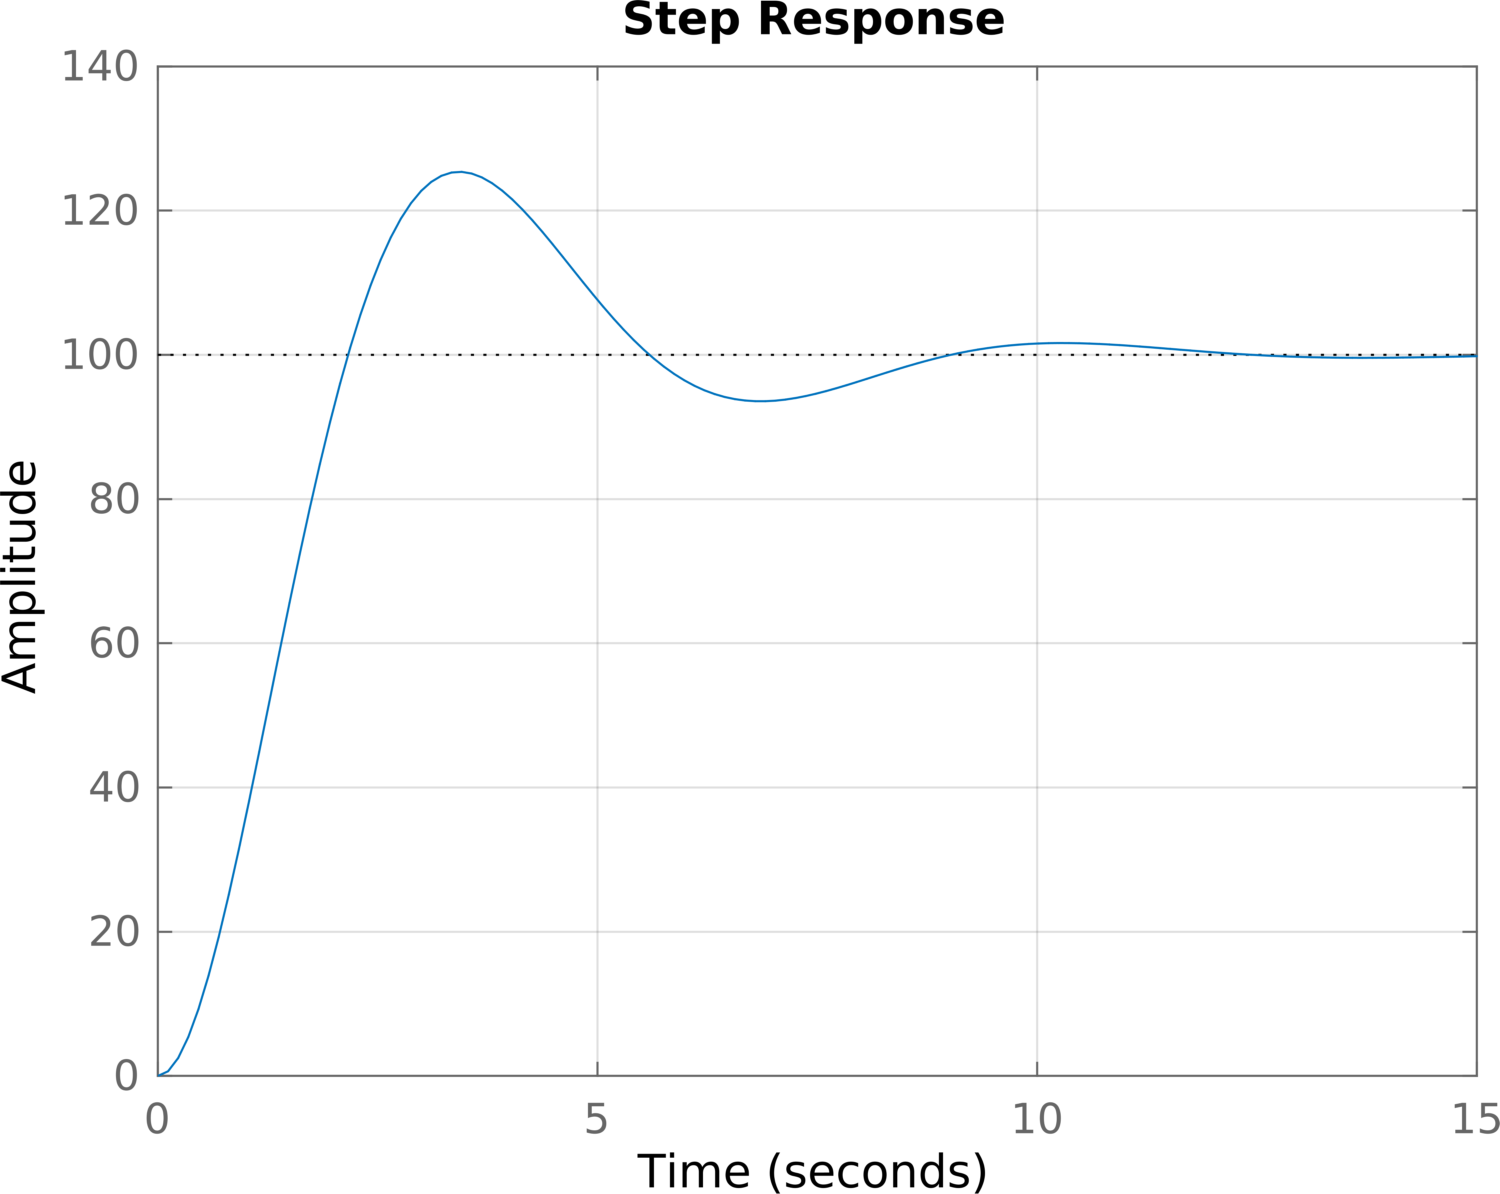
\includegraphics[width=\linewidth]{step2.png}
  \caption{Example unit-step response.}
  \label{f:step2}
\end{subfigure}%
\begin{subfigure}{.5\textwidth}
  \centering
  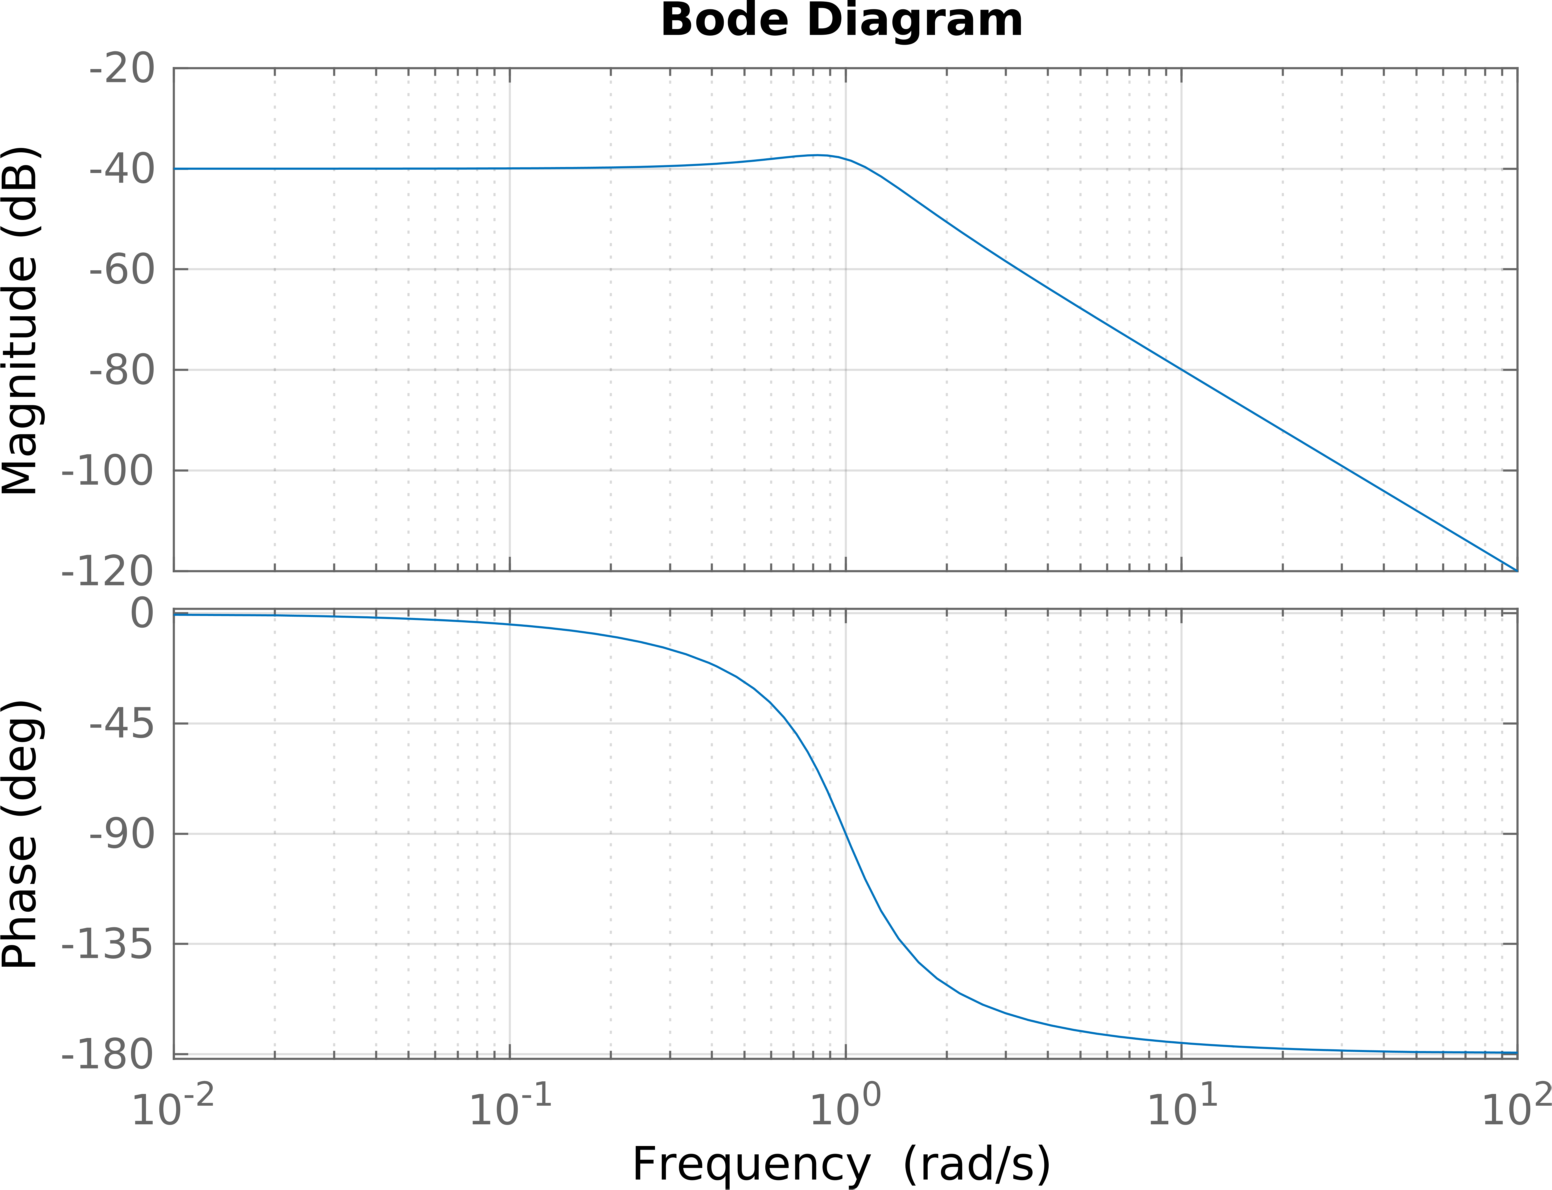
\includegraphics[width=\linewidth]{bode2.png}
  \caption{Example Bode plot}
  \label{f:bode2}
\end{subfigure}
\caption{Examples for exercises.}
\label{f:ex}
\end{figure}


%\section{Frequency Response Gain}
%The frequency response for a linear system consists of a magnitude and phase which are both dependent on frequency.  The Bode plot is a graph of both the magnitude and phase components.  



\end{document}
